\documentclass[a4paper,11pt]{article}
\usepackage[T1]{fontenc}
\usepackage[utf8]{inputenc}
\usepackage[francais]{babel}
\usepackage{lmodern}
\usepackage{amsmath}
\usepackage{graphicx}
\usepackage{multicol}
\usepackage{color}
\setlength\abovecaptionskip{0.10ex}
\RequirePackage{graphicx}
\DeclareGraphicsExtensions{.pdf,.jpg,.png,.JPG}
\RequirePackage{float}
\usepackage{titling}
\setlength{\droptitle}{-4cm}
\usepackage{fullpage}

\newcommand{\InsertFig}[1]{
\begin{figure}[H]
\begin{center}
\includegraphics[width=.75\textwidth]{img/#1}
\end{center}
\end{figure}}

\newcommand{\InsertFigTitle}[2]{
\begin{figure}[H]
\caption{#2}
\begin{center}
\includegraphics[width=.75\textwidth]{img/#1}
\end{center}
\end{figure}}


\title{Rapport SY09 TP02 - Classification automatique}
\author{Jean-Baptiste Audibert \& Yueqing Qin}
\date{\today} 

\begin{document}
\maketitle

\section{Classification hiérarchique}

\subsection{Etude des données mutations}

\noindent Pour étudier la classification hiérarchique, on va tout d'abord s'intéresser aux données \textit{mutations} qui représentent des distances génétiques entre des espèces. On réalise donc une \textbf{classification hiérarchique ascendante} pour les quatre critères d'agrégation présentés dans le cours de SY09 : \\

\begin{itemize}
\item Critère du lien minimum (on retient la distance minimum entre deux individus)
\item Critère du lien maximim ((on retient la distance maximum entre deux individus)
\item Critère du lien moyen (on retient la distance moyenne entre deux individus)
\item Méthode de Ward (on cherche à minimiser le critère d'inertie intra-classe) \\
\end{itemize}

\noindent On réalise donc ces classifications et on observe les quatre figures : 

\begin{figure}[H]
\begin{center}
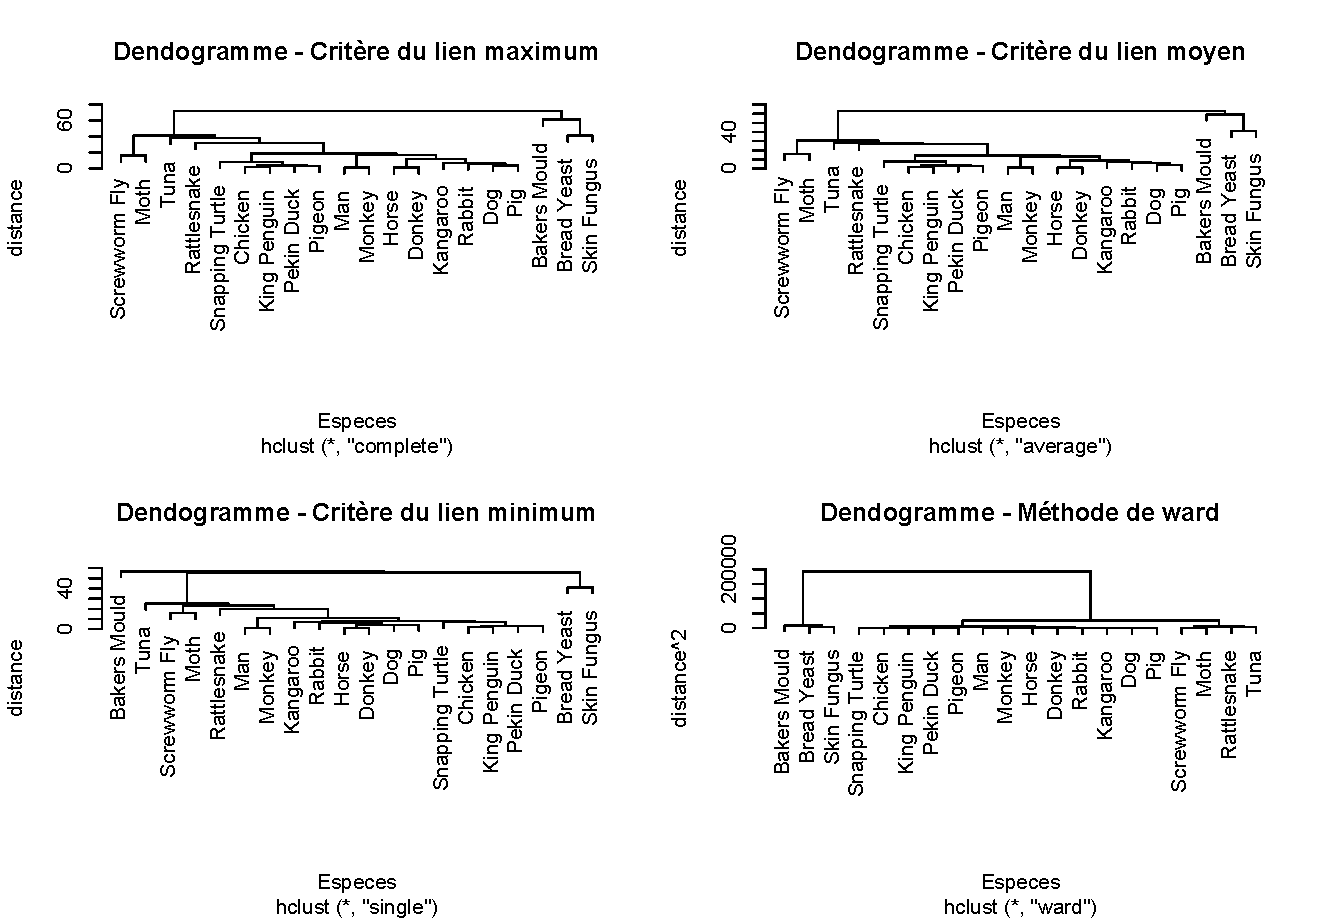
\includegraphics[width=.8\textwidth]{img/4dendo.pdf}
\end{center}
\end{figure}

\noindent On observe sur ces représentations l'émergence de deux groupes, un constitué de trois espèces (bakers mould, bread yeast, skin fungus), et un constitué des autres espèces. A l'intérieur de ce dernier, les sous-groupes diffèrent très peu selon la méthode utilisée. Il est donc difficile de proposer un critère optimal pour cette classification. Cependant, le critère du lien minimum sépare le groupe formé de trois espèces. On peut donc penser que ça ne peut être le critère optimal. De plus, la méthode de Ward peut être appliquée lorsque l'on est en présence d'un nuage de points. Hors ici on est directement en présence d'une matrice de distance et non de points à proprement parlé, donc ce critère n'est également pas valable pour cette étude.

\subsection{Etude des données Iris}

\noindent On s'intéresse à nouveau aux données \textit{iris}, déjà étudiées dans le TP1 sur l'ACP. Dans ce TP1, nous avions identifié trois groupes potentiels correspondant aux classes d'iris (\textit{Setosa}, \textit{Versicolor}, \textit{Virginica}) : 

\InsertFig{acpiris}

\noindent Par ailleurs, on peut noter que deux classes d'iris sont relativement proches, tandis que la dernière semble très éloignée des deux autres. 

\noindent Nous allons utiliser ici tout d'abord classification hiérarchique ascendante, afin de savoir, si l'on retrouve bien ces trois groupes. Le seul critère nous donnant un résultat exploitable est la méthode de Ward, car nous sommes dans un espace euclidien. Voici la représentation obtenue : 

\begin{figure}[H]
\begin{center}
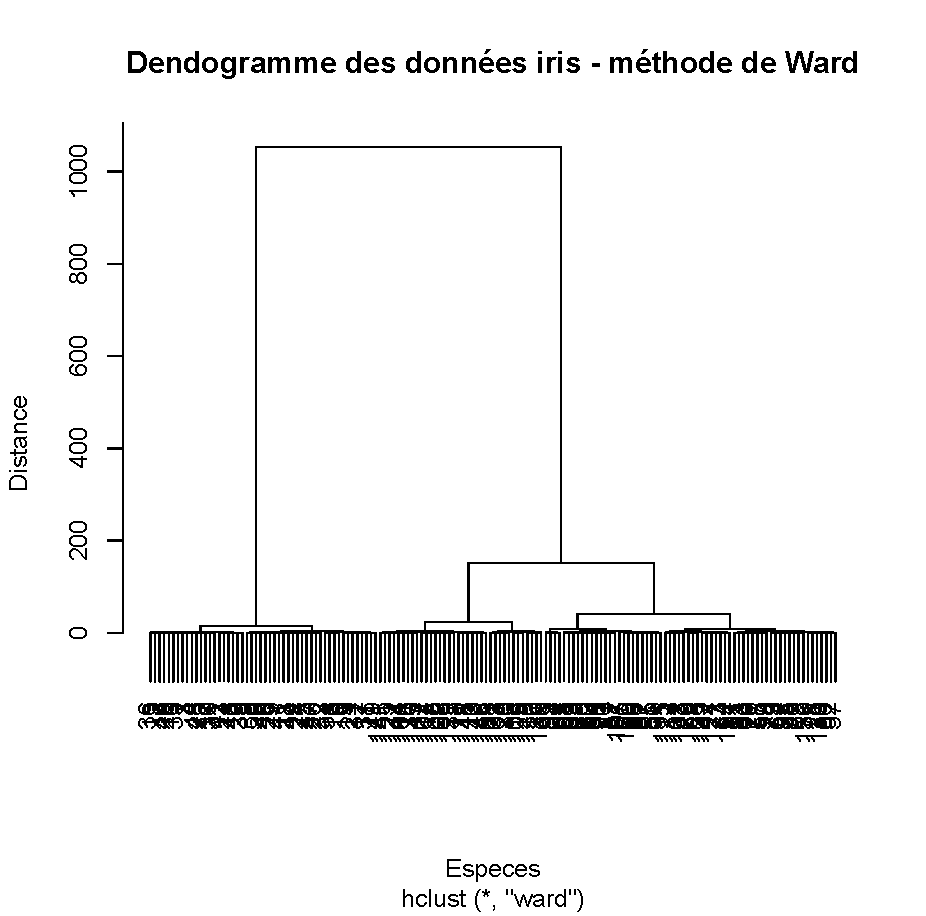
\includegraphics[width=.55\textwidth]{img/dendoiris.pdf}
\end{center}
\end{figure}

\noindent On observe ici bien trois groupes, correspondant aux trois groupes de l'ACP. De plus, on peut également voir la proximité entre deux des classes d'Iris. En effet,  on a un groupe \textit{seul}, sur la gauche du dendogramme, tandis que deux autres sont plus proches, avec des dissimilarités faible par rapport à la similarité entre les deux grands groupes ($\approx 200$ entre les deux groupes proches, $\approx 1000$ avec l'autre groupe).

\noindent Afin de continuer l'analyse, nous réalisons maintenant une classification hiérarchique descendante à l'aide de la fonction \textbf{diana}. On obtient le résultat suivant : 


\InsertFig{dendodiana}

\noindent On observe plus clairement les trois groupes, et à nouveau une proximité importante entre deux classes d'Iris.

\section{Les centres mobiles}

\noindent Dans cet exercice, nous allons utiliser l'algorithme des \textbf{centres mobiles} sur deux jeux de données déjà étudiés lors du TP sur l'ACP, les données \textit{iris}, et les données \textit{crabs}

\subsection{Données Iris}

\noindent On s'intéresse tout d'abord aux données \textit{iris}. On effectue des partitions en $K \in \{2,3,4\}$ classes. On en tire des des tableaux de contingences que l'on représente à l'aide d'histogrammes. On retrouve sur cet histogramme les \textcolor{red}{Setosa}, les \textcolor{green}{Versicolor} et les \textcolor{blue}{Virginica}

\begin{figure}[H]
\begin{center}
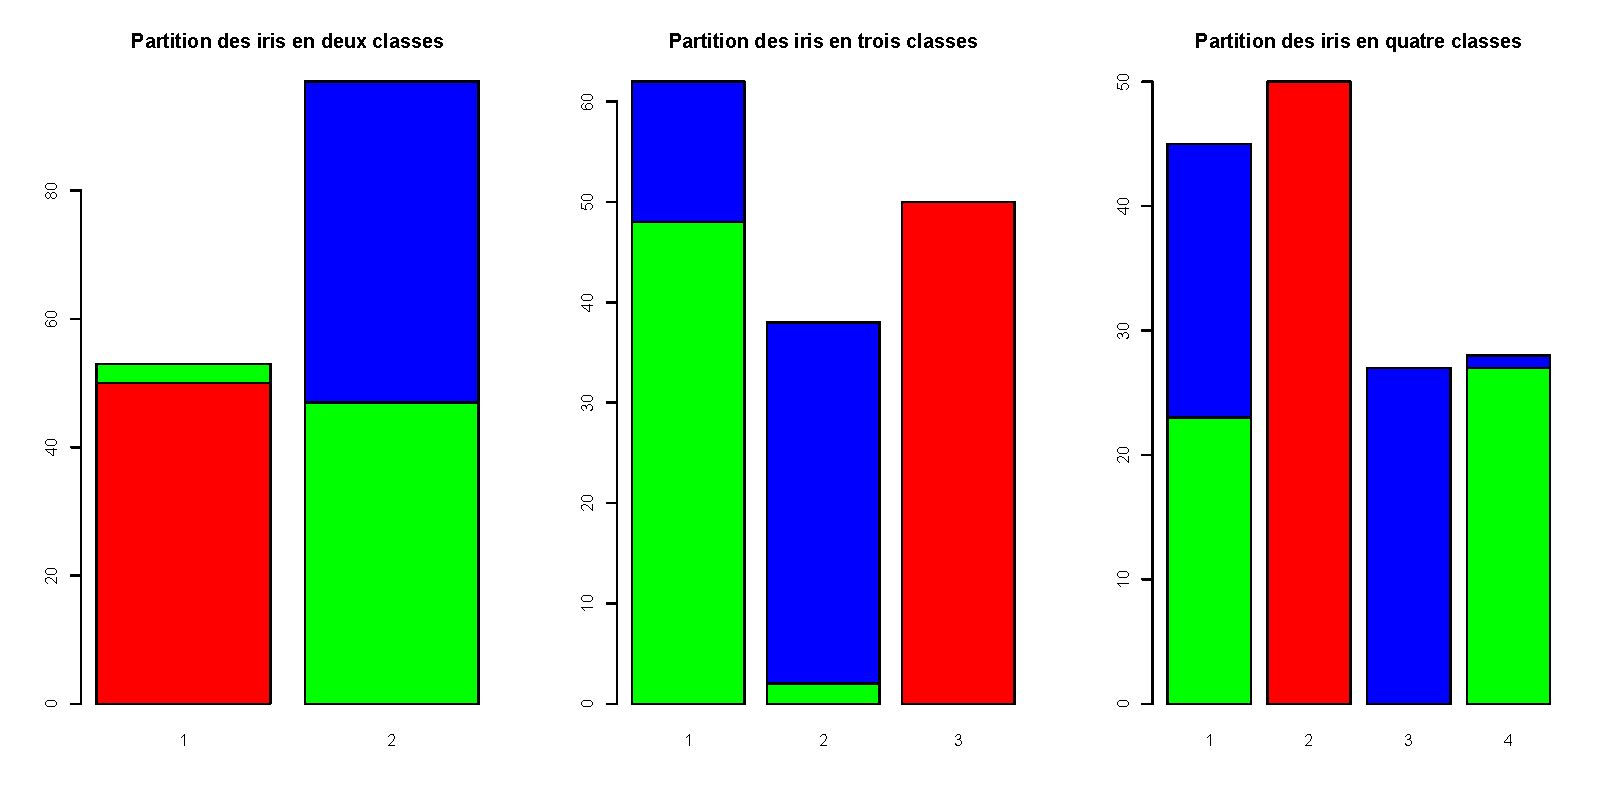
\includegraphics[width=\textwidth]{img/partiris}
\end{center}
\end{figure}

\noindent Lors de la partition en deux classes, on observe une classe constituée quasiment uniquement de \textcolor{red}{Setosa}, et une constituée de \textcolor{green}{Versicolor} et de \textcolor{blue}{Virginica}. C'est conforme à ce que l'on observait à la fois sur la projection du premier plan factoriel, et sur le dendogramme.
\noindent Sur la partition en trois classes, on a cette fois une classe seulement composée de \textcolor{red}{Setosa}, et une quasiment uniquement constituée de \textcolor{blue}{Virginica}. La dernière contient à la fois des \textcolor{blue}{Virginica} et \textcolor{green}{Versicolor}, ces derniers présents en plus grandes quantités. On a donc une partition qui correspond grossièrement aux trois classes d'iris. Cependant, les Virginica et les Versicolor étant proches, il est parfois difficile de les différencier.
\noindent La dernière partition en quatre classes nous montre trois classes composées d'une seule espèce (quasiment..), et une constituée de \textcolor{blue}{Virginica} et de \textcolor{green}{Versicolor} qui sont proches. \\

\noindent Toutefois, ces résultats ne nous sont pas apparus directement. En effet, lors de différents essais de \textbf{kmeans}, on a parfois obtenu des tableaux de contingence (et donc des histogrammes) très différents. Ceci est due au fait que l'algorithme contient une part de hasard dans son déroulement. Lors de la première étape de l'algorithme, on tire \textbf{au hasard} un nombre de points correspondant au nombre de classes que l'on souhaite obtenir. Le fait que l'on tire au hasard ces points initiaux ne peut garantir que l'on converge vers une solution optimale. Cette algorithme n'est donc pas stable. C'est pourquoi une étude plus poussé est nécessaire pour déterminer le nombre de classes optimal. \\

\noindent Nous allons réaliser ceci en effectuant, pour $K$, nombre de classe, $K \in [2;9]$, cent classifications à l'aide de l'algorithme des centres mobiles.
\noindent Pour ce faire, nous avons réalisé une fonction qui permet d'effectuer les partitions, et de nous renvoyer, pour chaque $K$, l'inertie intra-classe minimale. On peut ainsi élaborer un graphique représentant cette inertie en fonction du nombre de classes : 

\begin{figure}[H]
\begin{center}
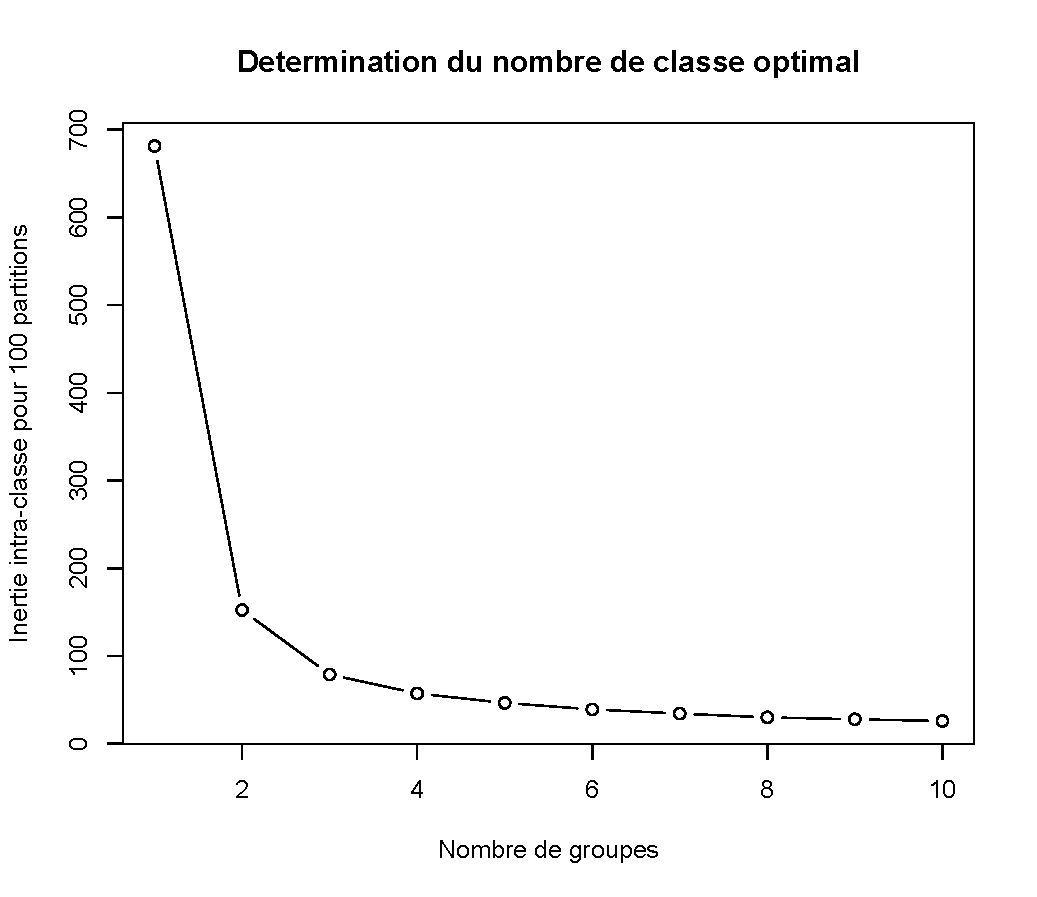
\includegraphics[width=.6\textwidth]{img/classeopt}
\end{center}
\end{figure}

\noindent Pour déterminer le nombre de classe optimal, on utilise la méthode du coude. Celle-ci nous dit que lorsque les variations de l'inertie intra-classe ne diminue plus significativement, on a atteint le nombre de classe optimal. Au vu du graphique, on peut ainsi dire que \textbf{le nombre de classe optimal est trois}. \\

\noindent Pour infirmer ou confirmer ces résultats, on réalise une \textit{partition réelle} des Iris à l'aide la C.A.H.

\noindent On réalise donc la C.A.H. sur les iris, on \textit{coupe} l'arbre de manière à répartir les iris en trois groupes, on dresse un tableau de contingence afin de connaitre la répartition des iris dans les classes selon leur espèce et on affiche un histogramme le représentant : 

\begin{figure}[H]
\begin{center}
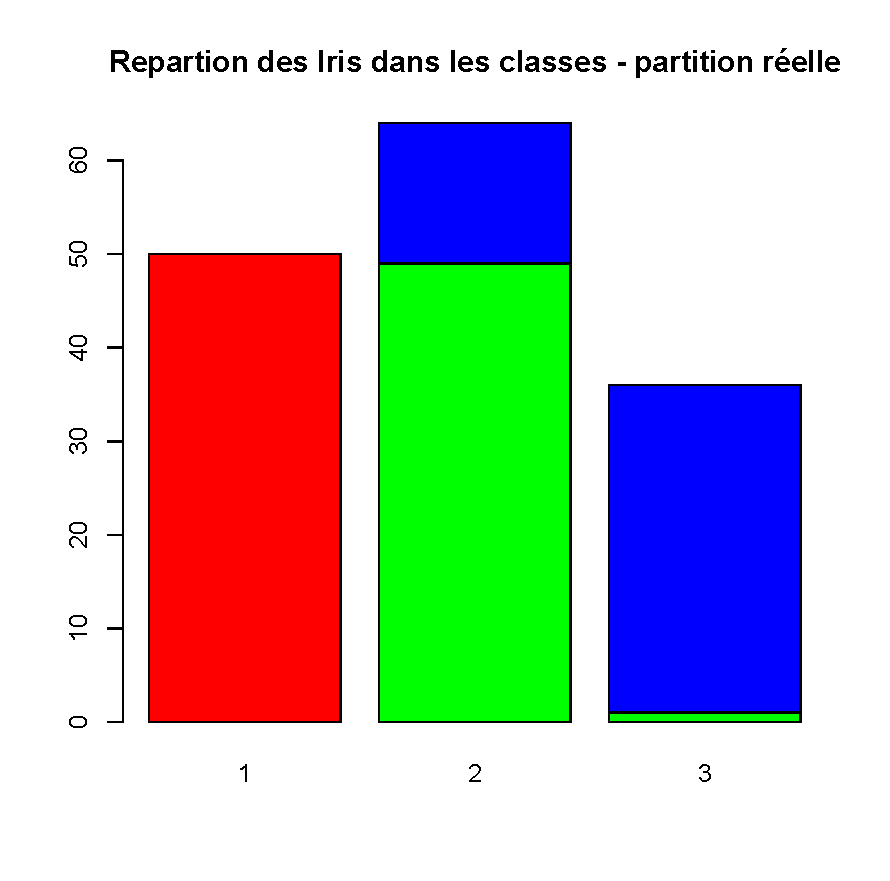
\includegraphics[width=.55\textwidth]{img/irispartreelle}
\end{center}
\end{figure}

\noindent On observe que les résultats semblent très proches voir similaires. Le nombre d'individus et la répartition dans les classes sont très quasiment égaux des résultats obtenus lors de la classification obtenue avec l'algorithme des centres mobiles.

\subsection{Etude des données crabs}

\noindent On s'intéresse désormais aux données crabs. On réalise tout d'abord la même étude, avec l'algorithme des centres mobiles, afin de connaitre le nombre de classe optimal, et de comparer avec ce que l'on obtient à l'aide de la classification hiérarchique ascendante.\\

\noindent On réalise 100 classifications pour $K$, nombre de classe, $K \in [2;9]$, et on représente l'inertie intra-classe en fonction du nombre de classe : 

\InsertFig{coudecrabs}

\noindent A l'aide de la méthode du coude, on peut ici dire que le nombre classe optimal est quatre, en effet, il semble raisonnable de dire qu'au delà de ce nombre, l'inertie intra-classe ne diminue plus significativement.

\noindent A quatre classes, on obtient la répartition suivante des crabes : 

\begin{figure}[H]
\begin{center}
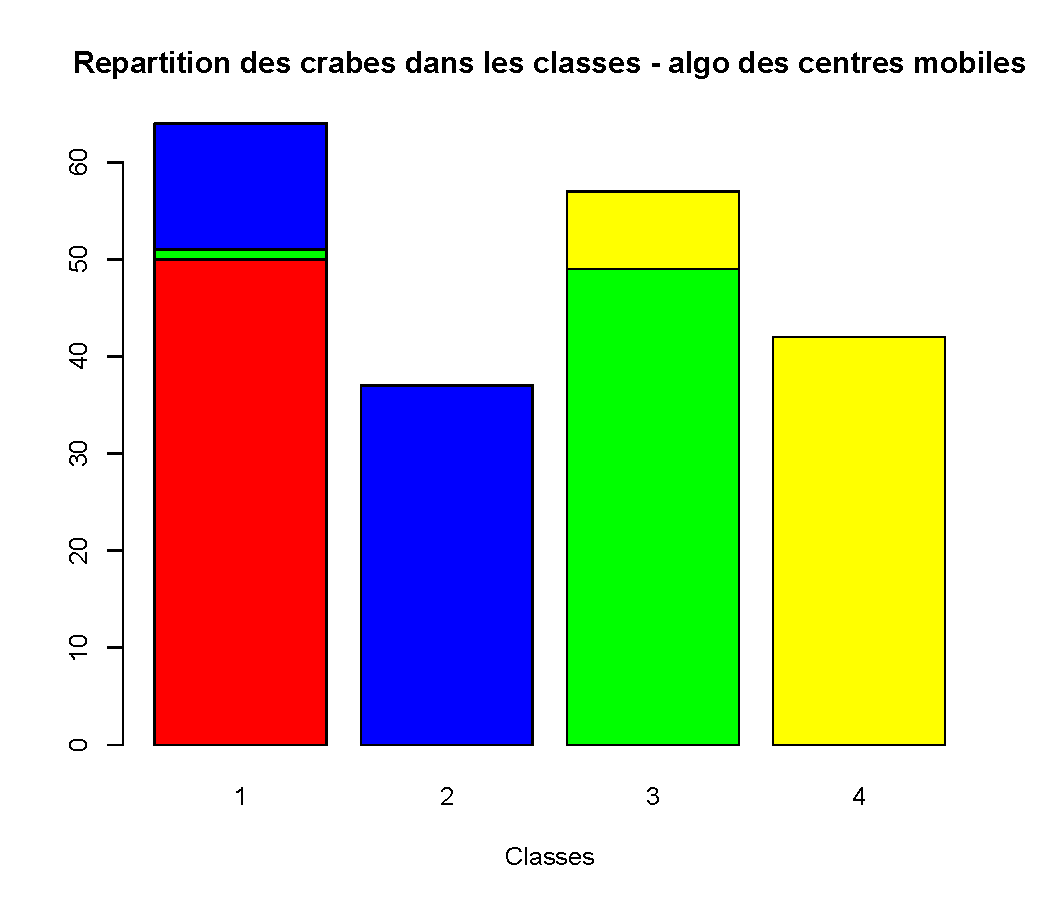
\includegraphics[width=.55\textwidth]{img/crabscm}
\end{center}
\end{figure}

\noindent On réalise désormais une classification hiérarchique ascendante sur ces données crabs. On utilise la méthode de Ward, qui encore une fois permet d'obtenir des résultats utilisables, car on est en présence d'un espace euclidien.. On coupe l'arbre en quatre classes, et on observe la répartition des crabes dans les classes : 

\begin{figure}[H]
\begin{center}
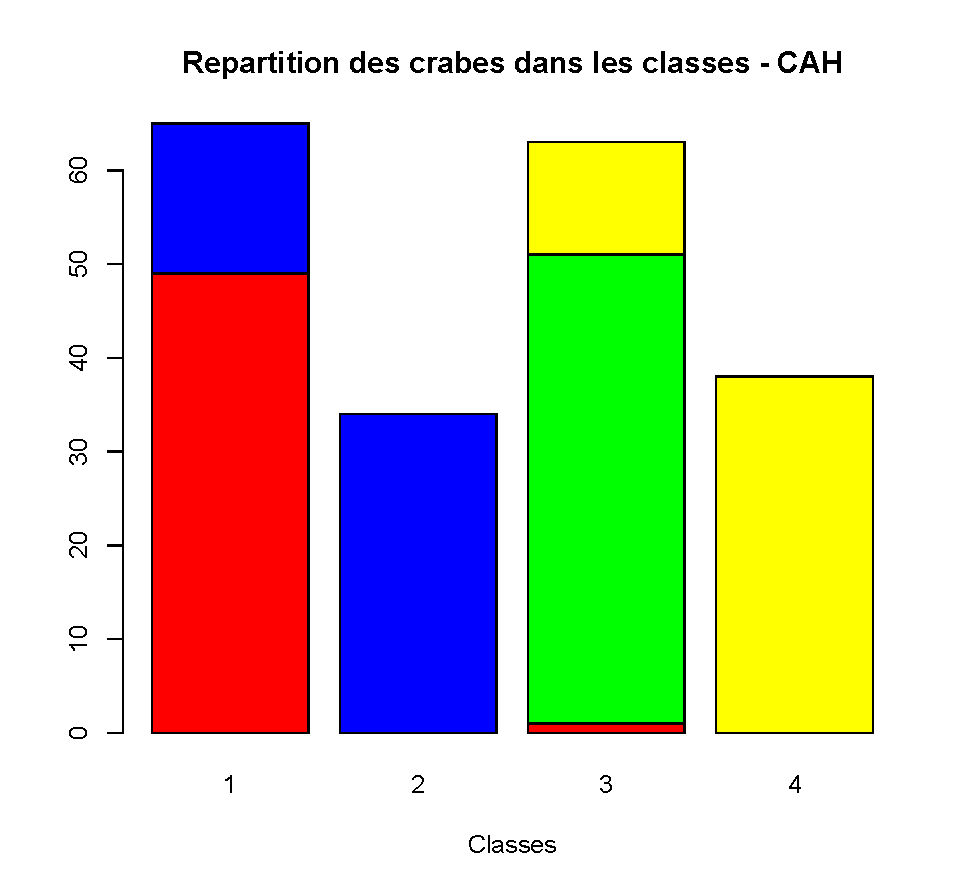
\includegraphics[width=.55\textwidth]{img/crabscah}
\end{center}
\end{figure}


\noindent On observe d'emblée une quasi-similarité. Afin d'affiner l'analyse, comparons les tableaux de contingence :

\begin{figure}[H]

  \begin{minipage}[b]{0.3\linewidth}
   \centering
   \caption{Tableau de contingence pour la CAH}
   \InsertFig{contigencearbrecrabs} 
  \end{minipage}
\hfill
  \begin{minipage}[b]{0.3\linewidth}
   \centering
   \caption{Tableau de contingence pour l'algorithme des centres mobiles}
  \InsertFig{contingencekmcrabs}     
  \end{minipage}

  \label{fig:ma_fig}

\end{figure}

\noindent On remarque que seulement 12 individus (sur 200), ne sont pas correctement classés. Soit un taux de reconnaissance de $94\%$, qui nous indique que l'algorithme des centres mobiles semblent aussi approprié qu'une partition réelle.

\section{Conclusion}

\noindent Dans ce TP, nous avons étudiés deux méthodes de classification : la partition réelle et la la partition à l'aide de la méthode des centres mobiles. Ces méthodes nous donnent des résultats globalement similaires même si parfois l'une est plus efficace que l'autre. Il faut ainsi adapter la méthode de classification (ainsi que le critère d'agrégation) en fonction des données, afin de s'approcher au maximum de la réalité.



\end{document}